\documentclass{../template/labo}
\usepackage[utf8x]{inputenc}

\usepackage[frenchb]{babel}
\usepackage[T1]{fontenc}

\usepackage{graphicx}
\usepackage{amssymb}
\usepackage{amsmath}
\usepackage{siunitx}
\usepackage{wasysym} %smiley
\usepackage{hyperref}% hyperliens
\usepackage{tikz}
\usetikzlibrary{babel,positioning,calc}
\usepackage{textcomp}
% \usepackage{minted}
\usepackage[long]{datetime}
\usepackage{gensymb} % \ohm, celsius
\usepackage{framed}
\usepackage{pdfpages}
\usepackage{todo}
\usepackage{paralist}
\usepackage{multicol}

\usepackage{mathastext} % math as standfard text : units are respecting typography conventions.
\usepackage{fancyhdr} %en-tête
\usepackage{qrcode}
\usepackage{pgfplots} %for latex grid
\usepackage{fontawesome}
\usepackage{gensymb} % \ohm, celsius



\usepackage{xspace} % typographie IN
\usepackage{hyperref}% hyperliens
\usepackage[all]{hypcap} %lien pointe en haut des figures
\usepackage[french]{varioref} %voir x p y
\usepackage{fancyhdr}% en têtes
%\input cyracc.def
\usepackage{pgfplots}
\usetikzlibrary{babel,positioning,calc}
\usepackage[americanresistors ]{circuitikz}
%\usepackage[]{gnuplottex}
\usepackage{ifthen}

\usepackage[]{pdfpages}
\usepackage[]{subfig}
\usepackage[]{attachfile}
\usepackage{qrcode}

%%%%%%%%%%%%
% Tables
%%%%%%%%%%%%
\usepackage{dcolumn}
\newcolumntype{.}{D{.}{.}{2}}
\usepackage{booktabs}
\renewcommand{\arraystretch}{1.1} % Opens up the table a tad
\usepackage{multicol}
\usepackage{multirow}



% \langexam{frenchb}
%
%\newboolean{koriG}
%\ifx\koriG\undefined
%\correction{false}
%\else
%\correction{true}
%\fi

\correction{false}
% \correction{true}

\author{The Fantastic Four}


%% fancy header & foot
\pagestyle{fancy}
\lhead{[ELEC-H-301] Électronique appliquée\\ LABO \no 2 : Montages à diodes \ifthenelse{\boolean{corrige}}{~-- corrigé}{}}
\rhead{v3.0.3\\ page \thepage}
\cfoot{}
%%

\pdfinfo{
/Author (The Fantastic Four, ULB -- BEAMS)
/Title (LABO 2 ELEC-H-301, Montages à diodes)
/ModDate (D:\pdfdate)
}

\hypersetup{
pdftitle={LABO 2 [ELEC-H-301] Électronique appliquée: Montages à diodes},
pdfauthor={The Fantastic Four, 2017 ULB - BEAMS  },
pdfsubject={Filtrage}
}


\begin{document}

\tptitle{}{Séance 2~: Montages à diodes}

\section{Introduction}

Les passages nécessitant des pré-déterminations ou des réflexions théoriques sont indiqués par un symbole \faCogs~ dans la marge,
ceux nécessitant de manipuler du matériel par le symbole \faFlask~ et les passages informatif par \faLightbulbO.


\subsection{But de la manipulation et objectifs d'apprentissage}
Cette manipulation a pour but d'illustrer :
\begin{itemize}
\item au niveau «application» : différents montages à diodes, aussi bien analogiques que numériques. 
\item au niveau «composant» : le fonctionnement des diodes les plus courantes : diode à jonction PN, diode Zener, LED.
\end{itemize}

À la fin de ce laboratoire, vous devez être capable :
\begin{itemize}
\item de dimensionner une résistance de limitation de courant pour une LED; 
\item d'utiliser la caractéristique d'une diode;
\item de dimensionner un circuit à simple alternance; 
\item de prévoir l'effet d'une charge sur un circuit à simple alternance;et 
\item de dimensionner des portes logiques avec des circuits à diodes; 
\item de dimensionner un circuit de protection à diode Zener ;
\item d'expliquer le fonctionnement des circuits comprenant des diodes (à jonction, LED, Zener, etc) ;
\item de lire la notice d'une diode et d'en extraire les informations utiles. 
\end{itemize}

\subsection{Prérequis}
\begin{itemize}
\item Circuit RC du premier ordre
\item Chapitre 5 du cours.\\ En particulier :
\begin{itemize}
\item caractéristique d'une diode
\item redresseurs simple alternance
\item polarisation d'une diode
\item diode Zener
\item LED
\end{itemize}



\end{itemize}


\subsection{Matériel}

\begin{center}
\begin{tabular}{p{0.2\textwidth}rlp{0.1\textwidth}}
	Composant & \multicolumn{2}{c}{Valeur} & Quantité \\\toprule
	\multirow{5}{*}{Résistance} & 100 & $\si{\ohm}$ & x1 \\
															& 150 & $\si{\ohm}$ & x1 \\
															& 330 & $\si{\ohm}$ & x1 \\
															& 1 & $\si{\kohm}$ & x1 \\
															& 10 & $\si{\kohm}$ & x3 \\\midrule
	\multirow{2}{*}{Capacités} 	& 10 & $\si{\nano\farad}$ & x1 \\
															& 1 & $\si{\micro\farad}$ & x1 \\\midrule
	Diode GP15B &   &   & x2 \\\midrule
	LED TLHR5400 &   &   & x1 \\\midrule
	Diode Zener 1N5226B-TR &   &   & x1 \\\midrule
	Interrupteurs JS202011CQN &   &   & x2 \\\bottomrule
\end{tabular}
\end{center}



\subsection{Prédéterminations}
Toutes les sections « prédétermination »  doivent être faites \textbf{avant} l'arrivée au laboratoire.

Le TP 4 portant sur les diodes fait également office de prédéterminations.
%Les prédéterminations des questions \ref{Q:1} à \ref{Q:predet} 

%\clearpage
\newpage
\pagestyle{fancy}


\section{Polarisation d'une diode, exemple de la LED}
Dans cette section, nous allons nous intéresser à la polarisation d'une diode afin de faire le lien entre les caractéristiques théoriques et l'utilisation pratique d'une diode.
\subsection{Caractéristique I/V théorique}
\subsubsection{Conventions}
Les conventions pour le tracé de caractéristique I/V pour les diodes sont «~courant positif de l'anode vers la cathode, convention récepteur~» :
\begin{figure}[h!]
	\begin{center}
		\begin{circuitikz}\draw
			(0,0) node[anchor=east] {A} to [short,i>^=$I$] (1.5,0)
			(0,0) to [Do, v<=$V$] (2.5,0) node [anchor=west]{K}
		;\end{circuitikz}
	\end{center}
\caption{Conventions électriques}
\label{fig:source}
\end{figure}

\marginpar{\color{white}6dd9a4cc75f4c05c00780b57a702246076eeab706d614a915428c03372ddf7ad445c006d38cedcd6a4749e838125d94a3fdff36a9131771074bc3c98df9b11c6}


\begin{figure}[h!]
	\vspace{-0.5cm}
	\begin{center}
		\subfloat[TLHR5401]{\href{http://www.vishay.com/docs/83012/tlhg540.pdf}{\qrcode[height=2.6cm]{http://www.vishay.com/docs/83012/tlhg540.pdf}}}\hspace{0.5cm}
		\subfloat[GP15B]{\href{https://www.vishay.com/docs/88638/gp15a.pdf}{\qrcode[height=2.6cm]{https://www.vishay.com/docs/88638/gp15a.pdf}}}\hspace{0.5cm}
		\subfloat[1N5226B-TR]{\href{https://www.mouser.be/datasheet/2/427/1n5221-1767759.pdf}{\qrcode[height=2.6cm]{https://www.mouser.be/datasheet/2/427/1n5221-1767759.pdf}}}\hspace{0.5cm}
	\end{center}\vspace{-0.5cm}
\caption{QR codes cliquables vers la documentation des composants}
\label{fig:}
\end{figure}


\subsubsection{Caractéristique I/V}
La caractéristique courant--tension théorique de la LED ressemble à la Figure~\ref{fig:carac_LED} :
\begin{figure}[h!]
	\vspace{-0.5cm}
	\begin{center}
	\ifthenelse {\boolean{corrige}} {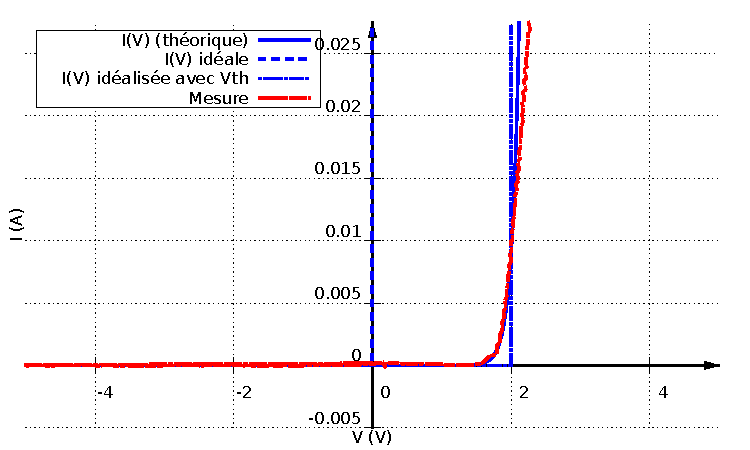
\includegraphics[width=\linewidth]{mesures/carac_mes.pdf}} {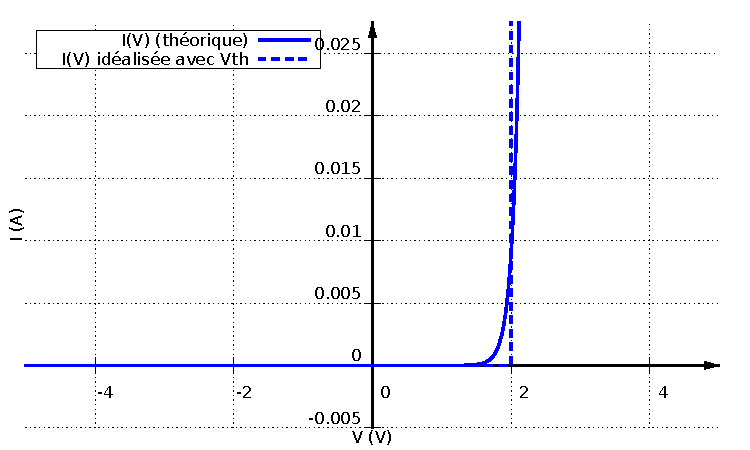
\includegraphics[width=12cm]{figures/carac.pdf}}
	\end{center}\vspace{-0.5cm}
\caption{Caractéristique I/V de la LED}
\label{fig:carac_LED}
\end{figure}	

\subsection{Mesure de points de fonctionnement}

Soit le montage de la Figure~\vref{fig:circuit_led}.
\begin{figure}[h!]
	\begin{center}
	\shorthandoff{:!}
		\begin{circuitikz}\draw
			(0,3) to [american voltage source, l=$V_{dc}$] (0,0)
			(0,3) to [european resistor, l^=$R$] (3,3)
			to [leDo] (3,0) -- (0,0)
		;\end{circuitikz}
	\shorthandon{:!}
	\end{center}
\caption{Diode polarisée en direct si $V_{dc}>0$}
\label{fig:circuit_led}
\end{figure}


\begin{manip}
	
\textit{Cette partie du laboratoire est à réaliser sur le protoboard en utilisant l'alimentation continue $5V$.}

\begin{astuce}
	La patte la plus longue de la LED est sa borne positive, son anode.
	De plus, le côté de la LED est plate du côté de la cathode.
\end{astuce}


	
\Question
{\label{Q:1}
	En prenant $R=\lbrace 100, 150, 330, 1000, \infty \rbrace \Omega$ et la tension de seuil indiquée dans la documentation de la LED \href{http://www.vishay.com/docs/83012/tlhg540.pdf}{TLHR5401} ($V_F$), mesurez et placez les cinq points correspondants sur le graphe de la Figure~\vref{fig:carac_LED}. Utilisez le protoboard et $V_{dc}=5V$.

	\begin{astuce}
		L'oscilloscope ne fonctionnant pas en ampèremètre, mesurez la tension aux bornes de la résistance et utilisez la loi d'Ohm pour en déduire le courant.
	\end{astuce}
}
{
\begin{center}
	\begin{tabular}{ccc}
		Résistance & $V_D$ & $I_D$ \\\toprule
		$100 \si{\ohm}$ & $2.25 \si{\volt}$ & $26.6 \si{\milli\ampere}$ \\\midrule
		$150 \si{\ohm}$ & $2.14 \si{\volt}$ & $18.9 \si{\milli\ampere}$ \\\midrule
		$330 \si{\ohm}$ & $2.00 \si{\volt}$ & $9.3 \si{\milli\ampere}$ \\\midrule
		$1000 \si{\ohm}$ & $1.84 \si{\volt}$ & $3.3 \si{\milli\ampere}$ \\\midrule
		$\infty$ & $0 \si{\volt}$ & $0 \si{\milli\ampere}$ \\\bottomrule
	\end{tabular}
\end{center}
}%R

\Question
{
	L'approximation I(V) idéalisée avec seulement la tension de seuil est-elle une bonne approximation ?
}
{On obtient quatre tensions différentes, donc l'approximation n'est pas parfaite.
Elle est néanmoins suffisante pour la suite des exercices.}%R
	\label{Q:2}

\Question
{
	Indiquez l'état de la diode sur le graphe de la page précédente en fonction de I.
}
{Elle est bloquante pour une tension inférieure à $V_{th} = 2 V$, passante sinon.}
	\label{Q:3}
	
\Question
{
	En tenant compte de la réponse à la question 2, calculez la valeur de $R$ pour obtenir un courant de 20mA dans la LED.	
}
{$$R=\frac{V_{dc}-V_{th}}{I_D}=150\Omega$$}%R
	\label{Q:4}

\Question
{
	Que se passe-t-il si la diode est mise en inverse ($V_{dc}<0V$ ou diode inversée) ?  Que peut-on dire du courant la traversant (faire une mesure) ? Est-elle éclairée ?
}
{La led est en inverse et est éteinte. Le courant la traversant est très faible : $\approx 50\mu A$ }%R
	\label{Q:5}

\Question
{
	Quelles précautions doivent être prises lors du fonctionnement en direct ? Même question pour un fonctionnement en inverse.
}
{Le courant maximum ne doit pas être dépassé, il faut donc placer une résistance en série. En inverse, la tension d'avalanche ne doit pas être atteinte.}%R
	\label{Q:6}

\end{manip}





\clearpage
\section{Redressement simple alternance}
Nous allons nous intéresser à un montage qui permet de transformer un signal AC (alternatif) en un signal DC (continu). Ce type de montage est un élément central qui permet de transformer le 220V alternatif (qui sort de votre prise) en 5V continu (que vous utiliser pour recharger vos appareils électroniques). 

\textit{Cette partie du laboratoire est à câbler sur le protoboard. Utilisez le générateur comme source alternative pour votre montage \textbf{sans utiliser l'alimentation continue 5V}.}


Voici le schéma d'un redresseur simple alternance :
\begin{figure}[h!]
	\begin{center}
		\begin{circuitikz}\draw
			(0,0) to [sV, l=$V_{ac}$] (0,3)
			to [Do] (3,3)
			to [european resistor,l_=$Z_{Charge}$] (3,0) to (0,0)
			(3.5,3) to [open, v^<=$V_{charge}$] (3.5,0)
			(3,3.2) to [open, v=$V_D$] (0,3.2)
		;\end{circuitikz}
	\end{center}
\caption{redresseur simple alternance}
\label{fig:red-simple-alt}
\end{figure}

\subsection{Prédéterminations}
\begin{predet}
\Question
{
	Tracez les tensions $V_{ac}$, $V_{charge}$ et $V_D$. Précisez l'état de la diode. Utilisez une tension de seuil de 1V pour simplifier (\textit{cf} \href{https://www.vishay.com/docs/88638/gp15a.pdf}{documentation GP15B}).%\marginpar{donner un graphe ???}
}
{Courbes $V_{ac}$ et $V_{ch}$ du graphe précédent.}%R
	\label{Q:7}

\Question
{
	Tracez sur un même graphe l'allure du courant circulant dans le circuit en fonction du temps.
}
{Courbe rouge $I_{ch}$\\
	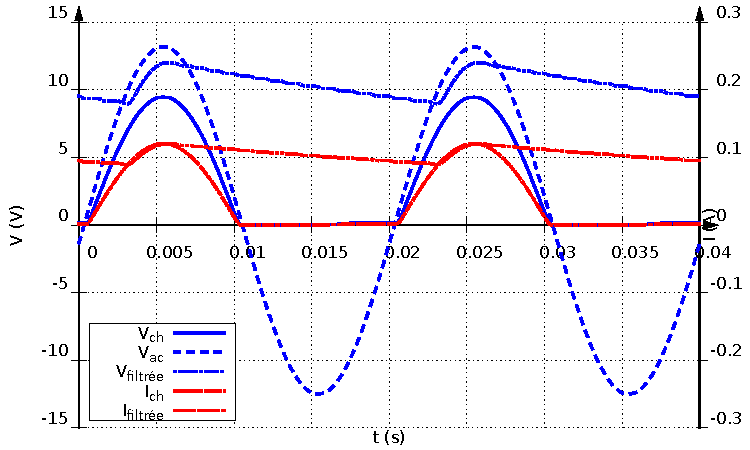
\includegraphics[width=\linewidth]{mesures/simple_alternance.pdf}
	Note : ces courbes ont été tracées pour une tension $V_{ac}$ plus élevée que votre montage, mais les allures relatives restent d'application.}%R
	\label{Q:8}

\Question
{
	La tension de sortie $V_{charge}$ est-elle stable, continue ? Que proposez-vous comme solution pour augmenter cette stabilité ?
}
{Non, ajouter une capacité de filtrage.}%R
	\label{Q:9}
\end{predet}

\subsection{Manipulation}
\begin{manip}
\Question
{
	Connectez le montage de la Figure~\ref{fig:red-simple-alt}. Utilisez comme source un signal de 100~Hz et d'amplitude 2V. Utilisez une résistance de $10 \si{\kohm}$ comme charge. Vérifiez vos prédéterminations expérimentalement (Attention à la polarité de votre diode).
	\begin{astuce}
		La bague argentée de la diode indique sa borne négative, sa cathode.
	\end{astuce}
}
{
	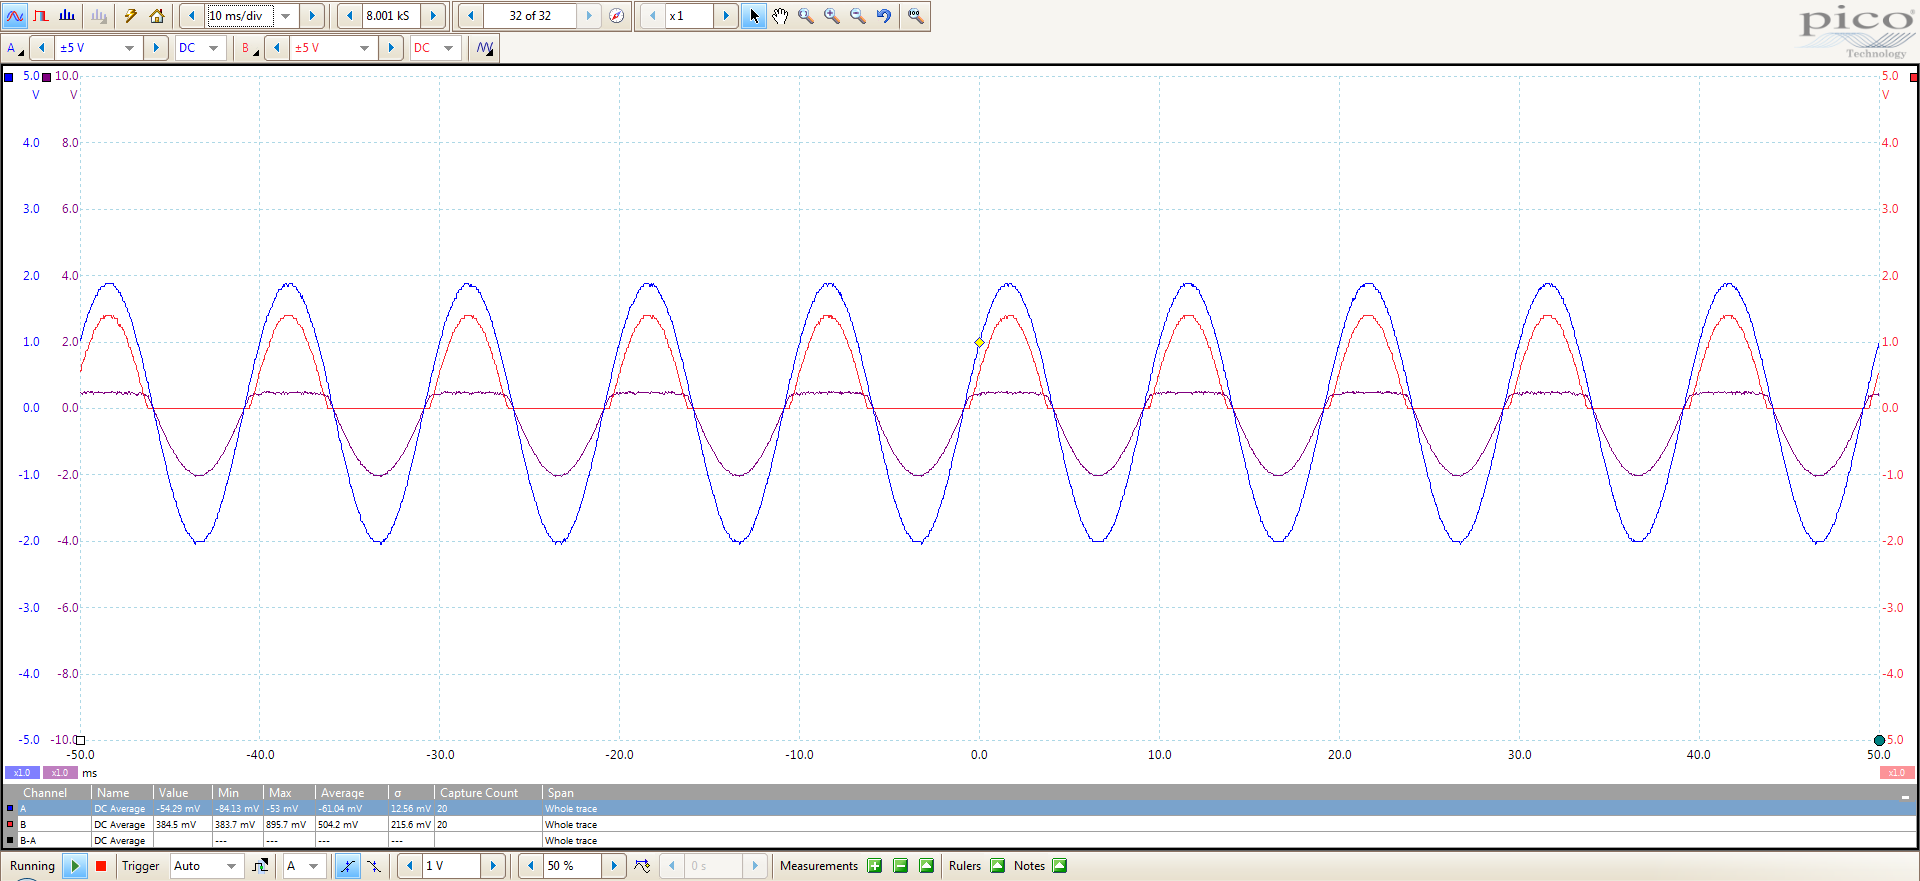
\includegraphics[width=\linewidth]{figures/redresseur_10k.png}
	Attention, si on utilise une charge trop faible, la résistance de sortie de $600\si{\ohm}$ du générateur n'est plus négligeable.
}
\end{manip}




\clearpage
\section{Filtrage capacitif}

Effectuons un filtrage capacitif\footnote{Il est également possible d'effectuer un filtrage inductif pour limiter l'amplitude des pics de courant sur la source alternative mais ces phénomènes dépassent les limites de ce cours.} en ajoutant une capacité en parallèle avec la charge.

\begin{figure}[h!]
	\begin{center}
		\begin{circuitikz}\draw
			(0,0) to [sV, l=$V_{ac}$] (0,3)
			to [Do] (5,3)
			to [european resistor,l=$R_{Ch}$] (5,0) to (0,0)
			(4,3) to [eC,l_=$C$, *-*] (4,0)
			(6,3) to [open, v^<=$V_{charge}$] (6,0)
		;\end{circuitikz}
	\end{center}
\caption{Redresseur simple alternance}
\label{fig:source}
\end{figure}


\subsection{Prédéterminations}

\begin{predet}
\Question
{
	Justifiez la polarité utilisée pour la capacité.
}
{Redresseur simple alternance, tension positive à la cathode par rapport à la charge.}%R
	\label{Q:10}

\Question
{
	%Q
	Tracez l'allure de $V_{charge}$ en tenant compte de la capacité.
}
{
	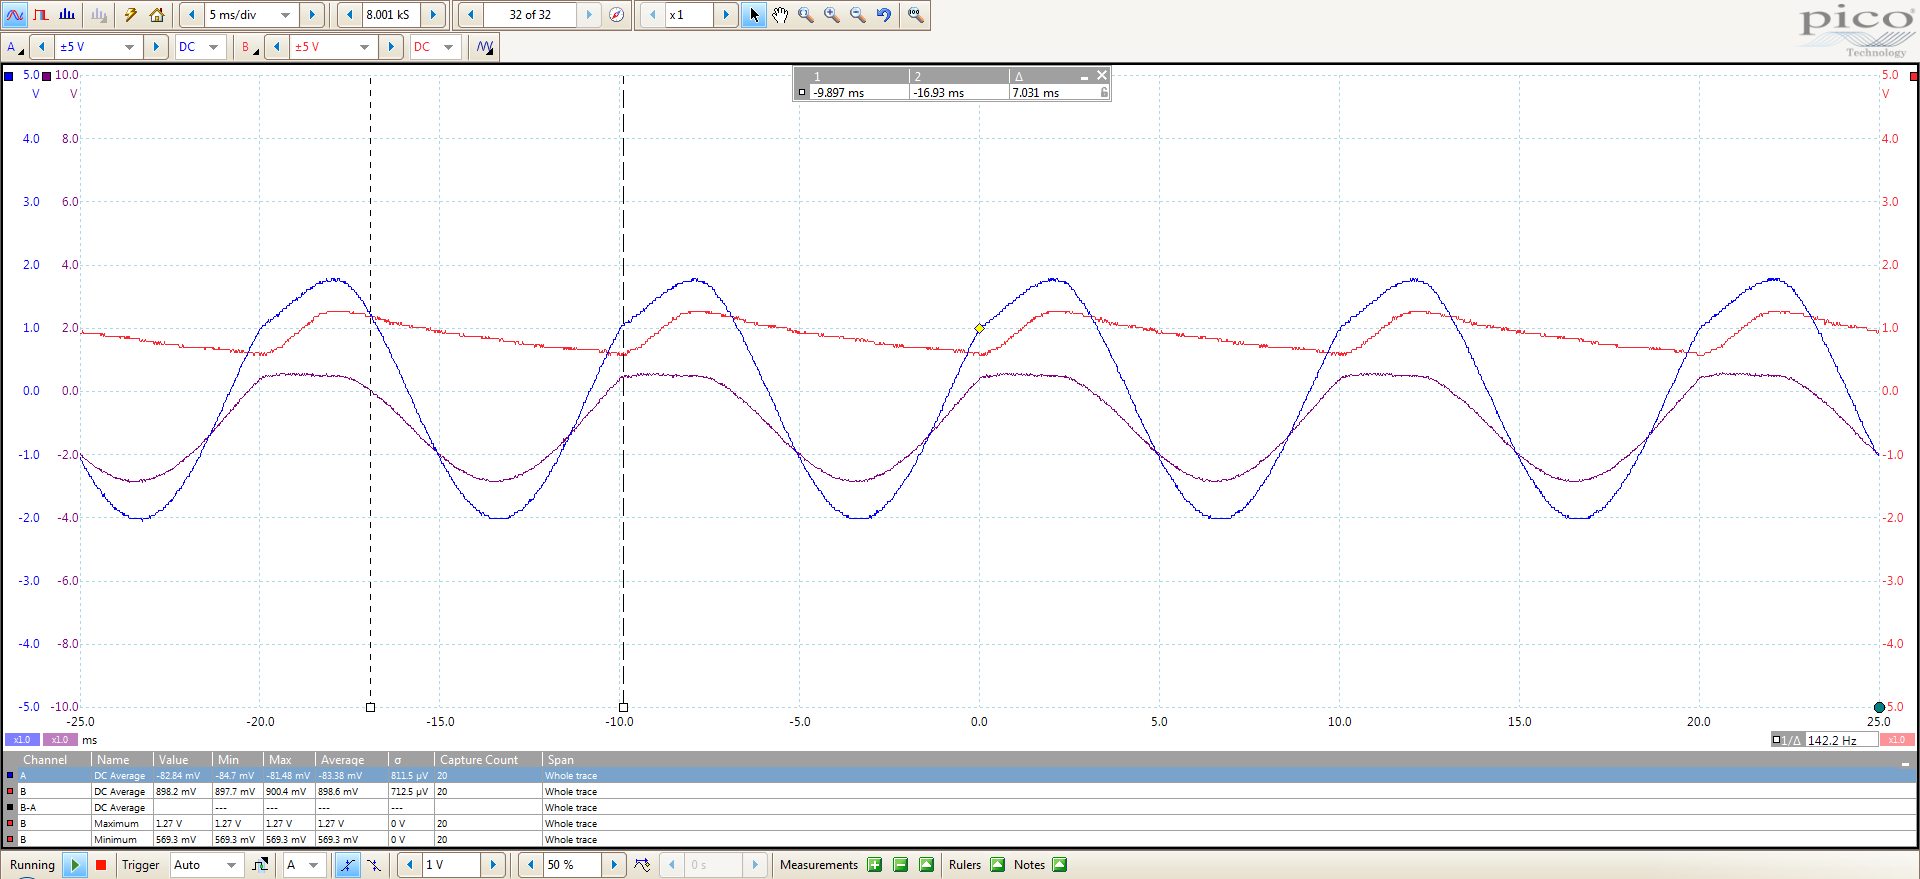
\includegraphics[width=\linewidth]{figures/redresseur_10k_filtre.png}
}%R
	\label{Q:11}


\Question
{
	Tracez l'allure du courant circulant dans la charge. Indiquez les intervalles de charge et de décharge.
}
{}%R
	\label{Q:12}
\end{predet}

\subsection{Manipulation}

\begin{manip}
\Question
{~\\
\begin{itemize}
\item Vérifiez expérimentalement. (\textbf{ATTENTION} à la polarité de votre condensateur).
\begin{astuce}
	La patte \textit{positive} d'un condensateur polarisé est plus longue.
	De plus, le côté du composant le long de la borne \textit{négative} est estampillé de symboles \faMinus.
\end{astuce}
\item Placez une résistance de charge en parallèle avec le condensateur ; observez son effet sur $V_{charge}$ pour différentes valeurs.
\item Expliquez qualitativement l'influence de cette résistance sur l'allure de $V_{charge}$.
\item Remarquez que le signal comporte plusieurs «~phases~» successives.
\item Quelle est la forme d'onde dans chacune de ces phases ?
\end{itemize}

}
{On suit le sinus de la source durant la période de charge, tandis qu'on a une exponentielle décroissante durant celle de décharge.}%R
	\label{Q:13}
\end{manip}

\subsection{Calcul de l'ondulation}
On remarque que lorsque le circuit est chargé, la tension de sortie ondule. Quantifions cette ondulation en fonction des éléments du circuit.

La tension de sortie peut être décomposée en une composante continue et une composante alternative, d'où : $V=V_m+\Delta_V$

\begin{predet}
\Question
{
	Établissez une formule permettant d'estimer $\Delta_V=f(R,C, V_m,\dots)$. %\marginpar{manque ptet qques paramètres}
	
	Utilisez les approximations suivantes :
	\begin{itemize}
	\item $\Delta_V<<V_m$
	\item le temps de charge du condensateur est négligeable devant son temps de décharge.
	\item la décharge de la capacité est linéaire
	\end{itemize}
	\begin{astuce}
		Pensez à utiliser un développement de Taylor de la décharge du condensateur à différents instants.
	\end{astuce}
	\label{Q:form-deltaV}
}
{
Loi de décharge d'un condensateur : $V_c(t) = V_m e^{-t/RC}$. On peut en déterminer son approximation au premier ordre avec un développement Taylor~: $V_c(t) = V_m (1-\frac{t}{RC})$.
Ce qui nous intéresse, c'est uniquement «~l'ondulation~» $\Delta V$.
Nous avons ainsi~: 
\begin{align*}
\Delta V & = V_f - V_i \\
& = V_c(t_f) - V_c(t_i) \\
& = V_m (1-\frac{t_f}{RC}) - V_m (1 - \frac{t_i}{RC})\\
& = V_m (\frac{t_i - t_f}{RC}) \\
& = - V_m (\frac{\Delta t}{RC})
\end{align*}
}%R
	\label{Q:14}
\end{predet}

Cette formule permet de dimensionner la valeur de la capacité à utiliser pour lisser la tension de sortie pour limiter l'ondulation à une valeur donnée pour une charge donnée.

\begin{manip}
\Question
{
	Mesurez $\Delta_V$ et comparez à la valeur calculée pour les mêmes paramètres. Les approximations faites à la question~\ref{Q:form-deltaV} sont-elles valables, optimistes ou pessimistes ?
}
{
Pour le redresseur simple alternance, la fréquence est de 100~Hz, ce qui correspond à une prédiode $T$ de 10~ms.
En pratique, $\Delta t$ sera légèrement plus faible que $T$, étant donné qu'il y a une courte période de charge à soustraire.

Avec une charge de $10 \si{\kohm}$, un condensateur de $1 µF$, une amplitude maximale $V_m$ de $1.27 \si{\volt}$ et un $\Delta t$ de 7~ms, on obtient un $\Delta V$ de $0.889 \si{\volt}$, proche des $0.7 \si{\volt}$ mesuré.

% Avec une période réduite à 18~ms, on obtient des résultats plus proches de la réalité~: $5.78 V$ pour $180 \Omega$, $3.15 V$ pour $330 \Omega$ et $1.04 V$ pour $1 k\Omega$.

}%R
	\label{Q:15}
\end{manip}




\clearpage
\section{Circuits logiques à diodes}

En logique numérique, les tensions sont utilisées pour représenter des états logiques binaires, c'est-à-dire des bits ``1'' ou ``0''. En logique 5V, le bit ``1'' est représenté par une tension de 5V (ou proche), et le bit ``0'' est représenté par une tension de 0V (ou proche). Les montages de la Figure~\vref{fig:circuit_logique} représentent deux portes logiques de base, avec deux entrées et une sortie. Considérez une résistance de charge $R_L$ de $10$~k$\Omega$. 
\begin{figure}[h!]
	\begin{center}
		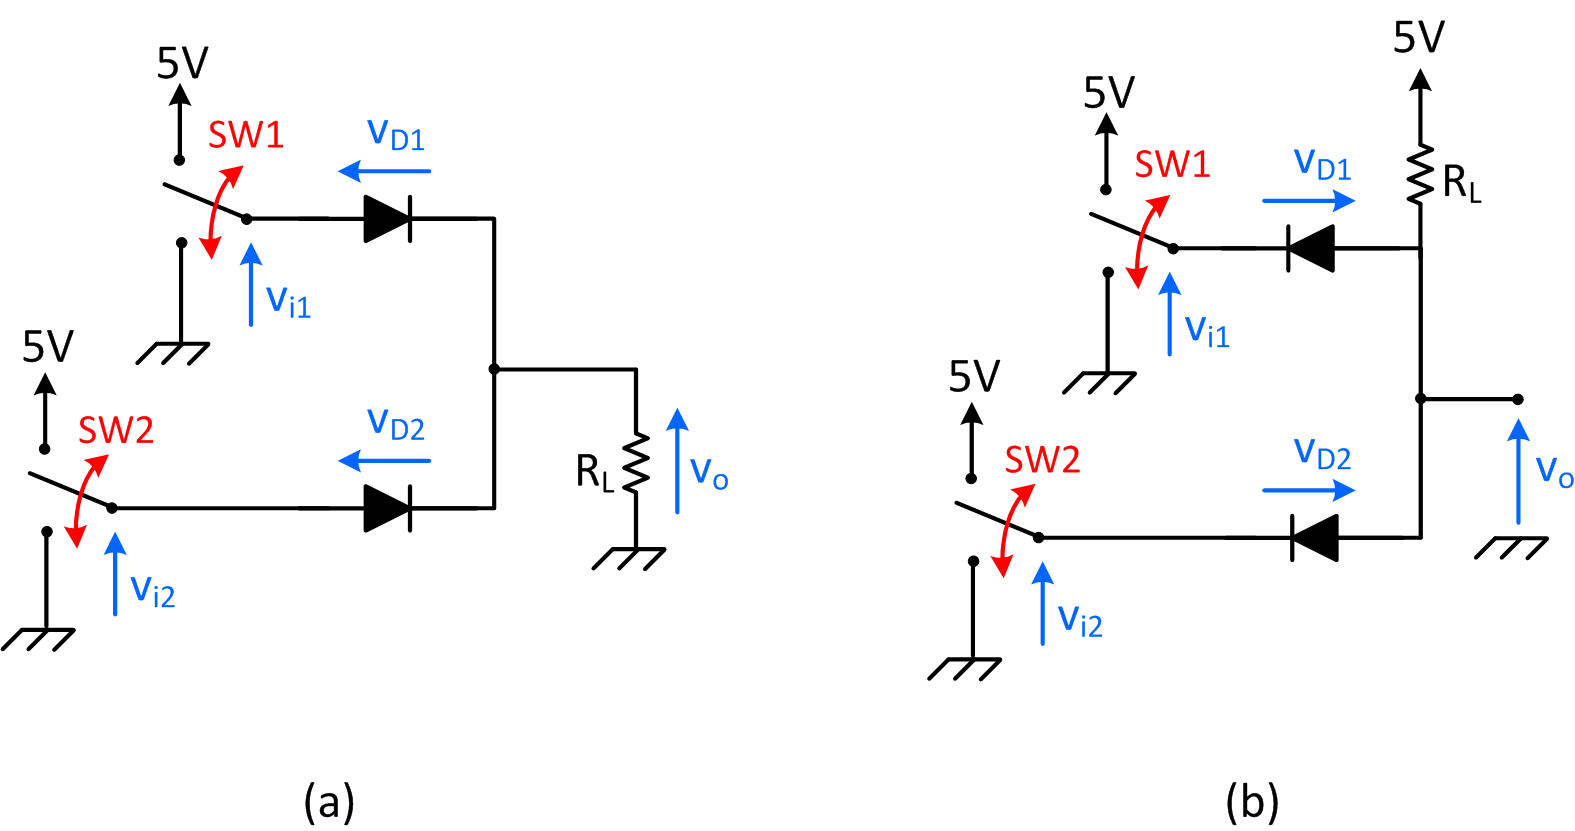
\includegraphics[scale=0.85]{figures/Circuits_logiques_diodes.png}
	\end{center}
\caption{Portes logiques à diodes}
\label{fig:circuit_logique}
\end{figure}


\begin{predet}

\Question
{	Pour le circuit de la Figure~\ref{fig:circuit_logique}-(a), déterminez l'état des diodes pour les différents états possibles des entrées. Calculez le courant qui passe dans chaque diode, ainsi que la tension de sortie. Considérez que la tension de seuil vaut $0.7$V. }
{Si un switch est connecté au 5V, la diode correspondante sera passante et la tension de sortie vaudra 4.3V. Le courant vaudra alors 4.3V/10k$\Omega$}
\label{Q:logique_1}
\Question
{	Pour le circuit de la Figure~\ref{fig:circuit_logique}-(b), déterminez l'état des diodes pour les différents états possibles des entrées. Calculez le courant qui passe dans chaque diode, ainsi que la tension de sortie. Considérez que la tension de seuil vaut $0.7$V. }
{Si un switch est connecté au 0V, la diode correspondante sera passante et la tension de sortie vaudra 0.7V. Le courant vaudra alors 0.7V/10k$\Omega$}
\label{Q:logique_2}
\Question
{	Quelle porte logique est implémentée par chacun des deux circuits? }
{(a) une porte OR et (b) une porte AND}
\label{Q:logique_3}
\Question
{	L'état haut et l'état bas à la sortie de ces circuits est-il bien à 5V/0V? Que pouvez-vous en conclure par rapport au seuil à utiliser pour les états logiques dans ces circuits? }
{Non, l'état haut du premier circuit est à 4.3V, et l'état bas du second circuit à 0.7V. Il faut donc prévoir un peu de marge pour la définition des états logiques (voir le concept d'immunité au bruit dans le chapitre 9.}
\label{Q:logique_4}

\end{predet}

\begin{manip}

\Question
{	Cablez le circuit de la Figure~\ref{fig:circuit_logique}-(a) et \ref{fig:circuit_logique}-(b), et vérifiez vos prédeterminations. }
{}
\label{Q:logique_5}
\Question
{	Si vous voulez connectez une LED pour indiquer l'état de sortie, comment devez-vous la connecter pour chacun des circuits? Changez la résistance de charge pour assurer une bonne illumination de la LED.  }
{(a) la LED doit être en série avec la résistance de charge et (b) la résistance doit être entre la sortie de $v_o$ et la masse. Il est intéressant de changer la résistance $R_L$ par une résistance de 100$\Omega$ afin d'avoir une bonne illumination. }
\label{Q:logique_6}

\end{manip}


\clearpage

\section{Circuit de protection à diode Zener}

Une diode Zener peut être utilisée afin de protéger un circuit. Imaginez le circuit de la Figure~\ref{fig:circuit_zener}. Le signal qui rentre dans le microcontrôleur doit être entre 0 et 3.3V, et la source est un signal alternatif de moyenne nulle et de fréquence 10~kHz. 
\begin{figure}[h!]
	\begin{center}
		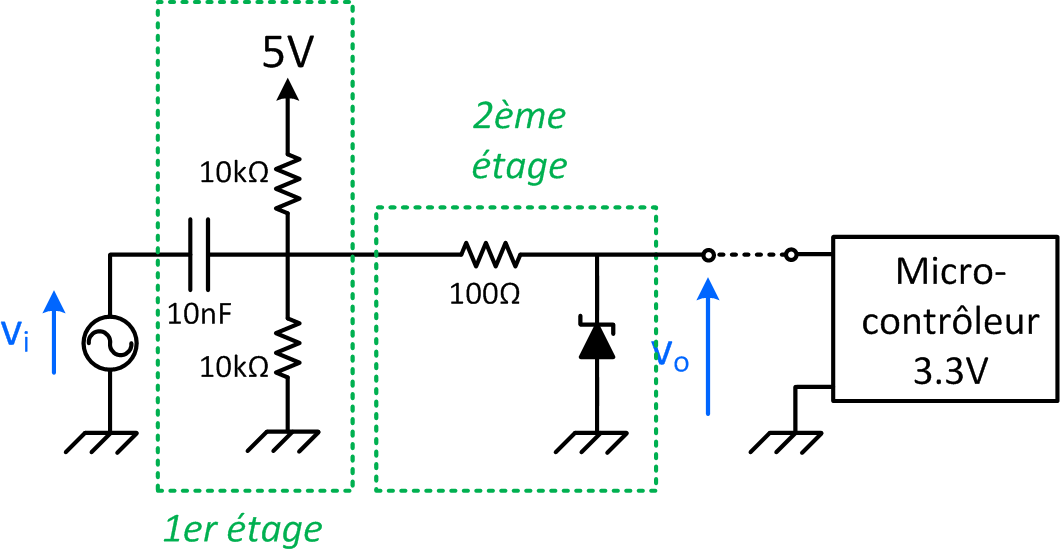
\includegraphics{figures/circuit_zener.png}
	\end{center}
\caption{Circuit de protection à diode Zener}
\label{fig:circuit_zener}
\end{figure}


\begin{predet}

\Question
{Le premier étage du circuit sert à rajouter une tension continue au signal d'entrée. En utilisant le principe de superposition, exprimez la tension à la sortie du premier étage du circuit. 

Vous pouvez condidérer que la capacité a une impédance nulle à la fréquence du signal alternatif, que la diode Zener est bloquante et qu'aucun courant n'entre dns le micro-contrôleur. }
{$v_{o1}=2.5+v_i$}
\label{Q:zener_1}
\Question
{Vérifiez dans les datasheets la tension d'avalanche de la diode Zener 1N5226B-TR. }
{Elle est de 3.3V}
\label{Q:zener_2}
\Question
{Le deuxième étage sert de circuit de protection. Dessinez le signal de sortie si le signal d'entrée est 
\begin{enumerate}
	\item une sinusoïde d'amplitude 2V à 10~kHz ;
	\item une sinuisoïde d'amplitude 0.5V à 10~kHz.
\end{enumerate}
}
{Le signal sera écrété vers le haut à 3.3V. }
\label{Q:zener_3}

\end{predet}
\begin{info}
	La résistance interne de la diode Zener ainsi que celle des connexions suffit à protéger la diode du courant qui la traverse lorsqu'elle est en avalanche.
\end{info}
\begin{info}
	L'étage suiveur permet de résoudre un problème d'adaptaion d'impédance entre l'étage 1 et l'étage 2. Sans celui-ci, lorsque la diode Zener est en avalanche, une partie non négligeable du courant du diviseur résistif circule au sein du deuxième étage, diminuant fortement la tension de décalage continue additionnée à $V_i$, et il n'est alors pas possible d'atteindre la tension d'avalanche de la Zener avec l'alimentation 5V.
\end{info}

\begin{info}
    Afin de réaliser l'étage suiveur, vous aurez besoin d'un amplificateur opérationnel TLV se trouvant dans le matériel du Labo 5. La Figure \ref{fig:tlv_suiveur} vous indique comment réaliser le cablage correspondant sans regarder dans les datasheets.
\end{info}

\begin{figure}[h!]
    \begin{center}
        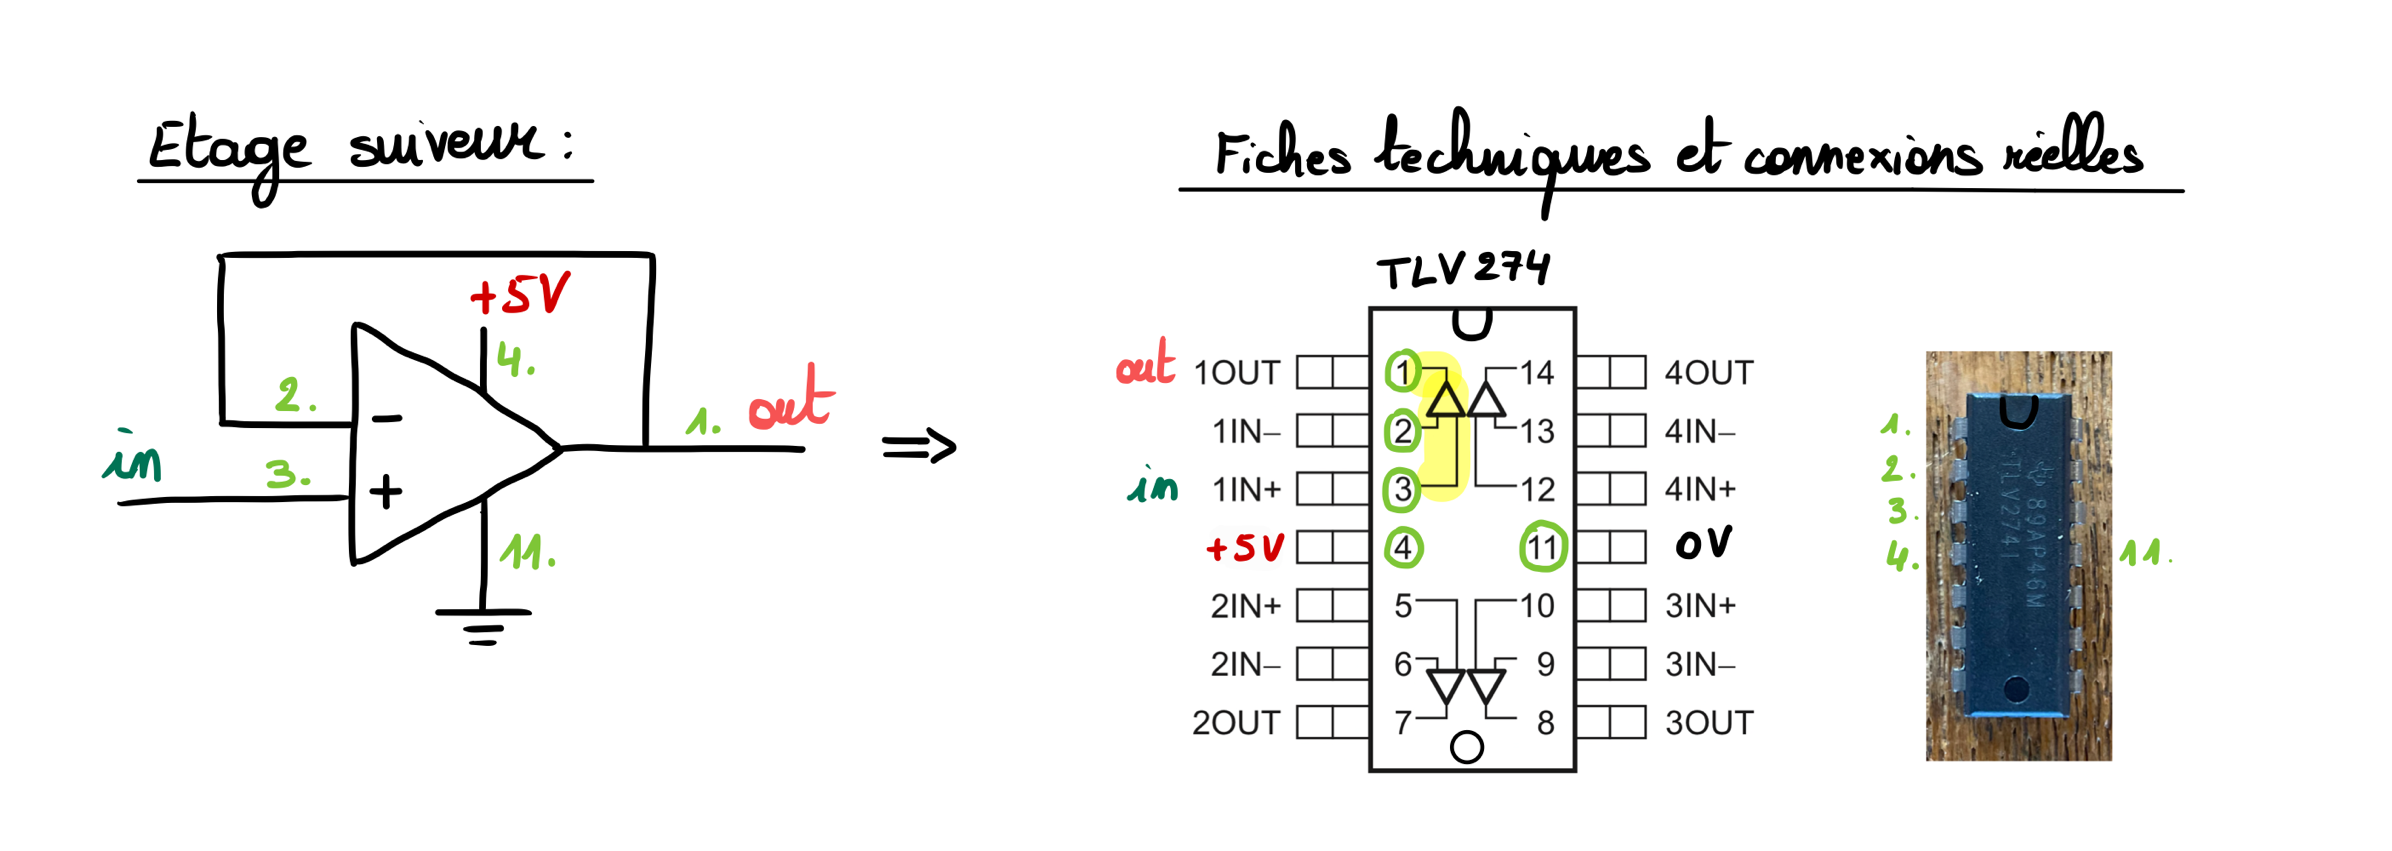
\includegraphics[scale=0.2]{figures/tlv_suiveur.png}
    \end{center}
    \caption{Cablage du TLV pour un montage suiveur}
    \label{fig:tlv_suiveur}
\end{figure}

\begin{manip}
\Question
{Câblez le circuit et vérifiez vos prédeterminations expérimentalement avec en entrée une sinusoide d'amplitude 2V. 
}
{On observe effectivement un écrêtage de la tension lorsque celle-ci est supérieure à 3.3V. }
\label{Q:zener_4}
\Question
{Si l'entrée est une sinusoïde d'amplitude 0.5V, observez-vous encore un écrêtage du signal? Si en aval on veut placer un microcontrôleur 3.3V, ce circuit fournit-il une protection efficace? }
{Le signal n'est plus écrêté. L'entrée du circuit est bien inférieure à 3.3V, mais n'exploite pas les tension au-dessus de 2.5V, ce qui peut être problématique. On peut envisager d'utiliser une Zener avec une tension Zener un peu plus élevée.
}
\label{Q:zener_4}
\Question
{Quelle est la limite {\bf inférieure} du signal de sortie. Adaptez le circuit pour pouvoir vérifier cette limite expérimentalement. Comment expliquez-vous cette limite inférieure? }
{La limite inférieure est à -0.7V, ce qui correspond à la tension de seuil de la diode Zener. }
\label{Q:zener_5}

\end{manip}


%Le circuit précédent produit une tension quasiment continue mais dont l'amplitude n'est pas précisément connue et peut varier assez fortement ($\pm 10\%$). Nous devons maintenant la réguler afin d'obtenir une tension continue de valeur connue indépendante des variations du réseau. Nous allons utiliser une diode Zener. D'autres composants permettant d'effectuer des régulations plus précises existent.
%
%\subsection{La diode Zener}%{\color{white}, sa vie, son œuvre\dots}
%
%La diode Zener utilise le phénomène d'avalanche existant d'une diode\footnote{Le phénomène d'avalanche n'est destructeur que si la température limite de jonction de la diode est atteinte. Généralement, l'entrée en avalanche donne lieu à la circulation d'un courant qui va échauffer très rapidement la diode et la détruire lorsque la température limite de jonction aura été atteinte.} dont le seuil a été fixé à la fabrication de la diode. Notez qu'une diode Zener  se comporte comme une diode classique si elle est utilisée en direct. Au risque de répéter un point important, une diode Zener s'utilise en \textbf{inverse} car sa caractéristique intéressante est son phénomène d'avalanche (en inverse).
%
%Les conventions électriques utilisées pour la diode Zener sont les mêmes que pour toute diode, pour rappel, 
%\begin{figure}[h!]
	%\begin{center}
		%\begin{circuitikz}\draw
			%(0,0) node[anchor=east] {A} to [short,i>^=$I$] (1.5,0)
			%(0,0) to [zDo, v<=$V$] (2.5,0) node [anchor=west]{K}
		%;\end{circuitikz}
	%\end{center}
	%\vspace{-0.4cm}
%\caption{Conventions électriques}
%\label{fig:zenerconv}
%\end{figure}
%\vspace{-0.4cm}
%sa caractéristique comporte un coude supplémentaire en inverse :
%\begin{figure}[h!]
	%\begin{center}
		%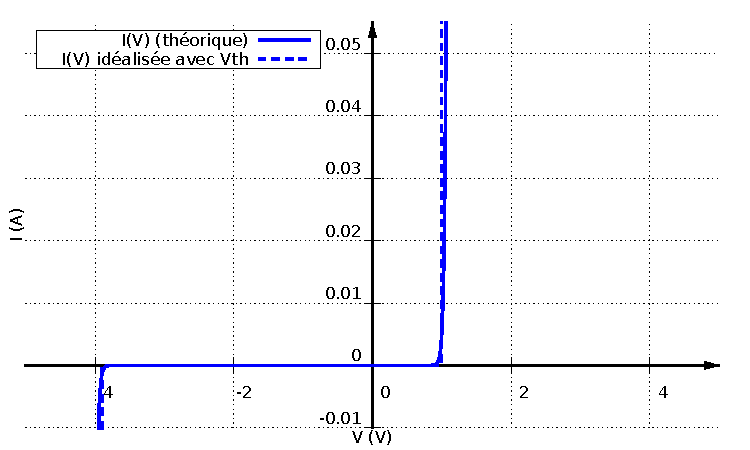
\includegraphics[width=10cm]{figures/carac_zener.pdf}
	%\end{center}
%\caption{Caractéristique I/V de la diode Zener}
%\label{fig:carac_Zener}
%\end{figure}
%
%Notez que la tension de Zener est positive et que sur la caractéristique, le phénomène d'avalanche se produit pour $V=-V_z$. Il faut donc utiliser la diode Zener en \textbf{inverse} pour pouvoir utiliser l'effet Zener. En direct, une diode Zener se comporte comme une diode commune ayant une tension de seuil de $0.7V$ généralement.
%
%\subsection{Utilisation en avalanche}
%Intéressons-nous uniquement à l'étage de régulation de l'alimentation présentée Figure~\vref{fig:alim} dans un premier temps.
%
%Soit le circuit de la Figure~\vref{fig:regulateur}.
%\begin{figure}[h!]
	%\begin{center}
		%\begin{circuitikz}\draw
			%(0,0) to [battery, invert, l=$V_{2}$] (0,3)
			%to [european resistor,l=$R$] (3,3)
			%(3,0) to [zDo, i<=$I_z$] (3,3)
			%(3,0) to (0,0)
			%(3,0) to [short,*-o] (4,0)
			%(3,3) to [short,*-o] (4,3)
			%(4,3) to [open,v^<=$V_{out}\equiv -V(Fig\ref{fig:zenerconv})$] (4,0)
		%;\end{circuitikz}
	%\end{center}
%\caption{Diode Zener utilisée en avalanche pour effectuer une régulation en tension}
%\label{fig:regulateur}
%\end{figure}
%
%\Question
%{
	%En supposant $V_2>V_{out}$, prédéterminez :
	%\begin{enumerate}
	%\item l'état de la diode Zener
	%\item la tension $V_{out}$
	%\item la valeur du courant traversant la diode $I_z$ %\marginpar{ajouter $I_z$ aux circuits}
	%\item les valeurs des puissances dissipées par les différents éléments du circuit
	%\end{enumerate}
%}
%{
%\begin{enumerate}
%\item En avalanche.
%\item $V_{out}$ = $V_z$
%\item $V_z = V_2 - V_R = V_2 - R\cdot I_z \Leftrightarrow I_z = \frac{V_2 - V_z}{R}$
%\item $P_R = V_R \cdot I_z = R\cdot I_z^2 = (V_2 - V_z)^2$ et $P_D = V_z \cdot I_z = \frac{V_z \cdot (V_2 - V_z)}{R}$
%\end{enumerate}
%}%R
	%\label{Q:21}
%
%
%\subsection{Influence d'une charge}
%Ajoutons une charge à ce beau circuit, nous obtenons :
%\begin{figure}[h!]
	%\begin{center}
		%\begin{circuitikz}\draw
			%(0,3) to [battery, v_<=$V_{2}$] (0,0)
			%(0,3) to [european resistor,l=$R$] (3,3)
			%(3,0) to [zDo, i<=$I_z$] (3,3)
			%(3,0) to (0,0)
			%(3,0) to [short,*-o] (4,0) to (5,0)
			%(3,3) to [short,*-o] (4,3) to [short, i=$I_{out}$] (5,3)
			%(5,3) to [european resistor,l=$R_{\mbox{ch}}$] (5,0)
			%(3.5,3) to [open,v^<=$V_{out}$] (3.5,0)
		%;\end{circuitikz}
	%\end{center}
%\caption{Circuit de régulation de tension, chargé}
%\label{fig:regul_charge}
%\end{figure}
%
%\newpage
%\subsection{Prédéterminations}
%%Le circuit alimente une charge qui consomme $I_{out}$.
%%Sachant que :
%
%\begin{itemize}
%\item $V_2 = 13V$
%\item $V_z = 9.1V$
%\item la puissance maximale que peuvent dissiper $R$ et la diode est $1W$.
%\end{itemize}
%%\subsubsection{Cas limites}
%\Question
%{
	%Indiquez l'état de la diode, exprimez et calculez $I_{\mbox{out}}$ et la puissance dissipée par les différents éléments ($R, D, R_{\mbox{ch}}$) dans les 3 cas suivants :
	%\begin{enumerate}
	%\item la charge est un court-circuit
	%\item la charge est un circuit ouvert
	%\item la charge est telle que le courant circulant dans la diode est négligeable devant les autres courants circulant dans le circuit.
	%\end{enumerate}
%}
%{
	%\begin{enumerate}
		%\item CC : $I_{out} = \frac{V_2}{R}$, $P_{\mbox{charge}}=0$, $P_R=V_2^2/R$, $P_D=0$, la diode est bloquante.
		%\item CO : $I_{out} = 0$, $P_{\mbox{charge}}=0$, $P_R=\left(V_2-V_z\right)^2/R$, $P_D=V_z\cdot \left(V_2-V_z\right)/R$, la diode en avalanche
		%\item $I_z\simeq 0$ : $I_{out} = \frac{V_2 - V_z}{R} = \frac{V_z}{R_{ch}}$ (on dimensionne la charge pour être dans ce cas limite), $P_{\mbox{charge}}=\frac{V_z\cdot \left(V_2-V_z\right)}{R}$, $P_R=\frac{\left(V_2-V_z\right)^2}{R}$, $P_D = V_z \cdot I_z \simeq 0$, la diode est tout juste en avalanche.
		%\end{enumerate}	
	%}%R
	%\label{Q:22}
%
%\Question
%{
	%%Calculez les valeurs numériques correspondant aux 3 cas de la question~\ref{Q:23b}. 
	%$R$ et $D$ ne doivent pas dissiper plus que leur puissance maximale admissible quelle que soit la charge. %, cela revient à choisir le cas le plus contraignant.
	%Les questions suivantes ont pour but de vous faire dimensionner la résistance $R$ afin de respecter ces contraintes.
	%\begin{enumerate}
	%\item Afin de déterminer ces puissances, doit-on considérer la diode Zener en avalanche ou bloquante~?
	%\item Pour quelle valeur de $I_{out}$ la puissance dissipée par la diode est-elle maximale ?
	%\item Pour quelle valeur de $I_{out}$ la puissance dissipée par la résistance $R$ est-elle maximale ?
	%\item Déduisez la valeur minimale de $R$ des 2 calculs précédents (tous les composants doivent survivre).
	%\item Quel est le courant maximum que ce circuit peut fournir à la charge (en méritant encore son nom de régulateur de tension, \textit{i.e.} avec une tension de sortie régulée) ?
	%\item Quelle est la résistance de charge correspondante ?
	%\end{enumerate}
%}
%{
	%\begin{enumerate}
	%\item Si la diode est bloquante, il n'y a aucune puissance produite ou consommée dans le circuit. Nous allons donc considérer que la diode est en avalanche.
%
	%\item $P_D = I_z \cdot V_z$, or $I = I_z + I_{out} = \frac{V_2 - V_z}{R} \Leftrightarrow I_z = I - I_{out} = \frac{V_2 - V_z}{R} - I_{out}$.
	%Ainsi, $P_D = V_z\cdot (\frac{V_2 - V_z}{R} - I_{out})$ est maximum lorsque $I_{out} = 0$.
	%
	%\item $P_R = V_R \cdot I = \frac{V_R^2}{R} = \frac{(V_2 - V_z)^2}{R}$, avec $V_z = V_{out} = R_{ch} \cdot I_{out}$, on obtient donc $P_R = \frac{(V_2 - R_{ch} \cdot I_{out})^2}{R}$.
	%Quand cette valeur est-elle maximale ?
	%\begin{itemize}
		%\item Lorsque $I_{out} = 0$, on se trouve alors dans le cas d'un circuit ouvert (sur la charge) et la diode sera forcément en avalanche.
		%Un bilan de puissance du circuit permet de mettre en évidence que la résistance $R$ \textit{et} la diode ont une puissance non nulle~: $P_{V_2} = P_R + P_{V_z} \Leftrightarrow \frac{V_2 \cdot (V_2 - V_z)}{R} = \frac{(V_2 - V_z)^2}{R} + \frac{V_z\cdot (V_2 - V_z)}{R}$.
		%\item Losque $R_{ch} = 0$, c'est-à-dire losque la charge est remplacée par un court-circuit.
		%La diode sera alors bloquante ($V_z = 0$) et la puissance dissipée dans la résistance sera de $\frac{V_2^2}{R}$, au lieu de $\frac{(V_2 - V_z)^2}{R}$ lorsque la diode est en avalanche.
		%Cette fois-ci, un bilan de puissance nous montre que la puissance de la source est entièrement dissipée dans la résistance $R$~: $P_{V_2} = P_{R}$.
		%C'est dans cette situation que la puissance dissipée par la résistance est maximale.
	%\end{itemize}
	%
	%\item En reprenant les résultats des deux questions précédentes, on peut mettre en évidence la puissance maximale dans la diode et dans la résistance.
%
	%$P_{D, max} = V_z \cdot \frac{V_2 - V_z}{R} \leq 1W \Leftrightarrow R \geq V_z \cdot \frac{V_2 - V_z}{1 W} = 35.49 \Omega$.
%
	%$P_{R, max} = \frac{V_2^2}{R} \leq 1W \Leftrightarrow R \geq \frac{V_2^2}{1W} = 169 \Omega$.
	%
	%\item Le circuit se comporte comme un régulateur lorsque la diode Zener limite la tension dans la charge, soit $V_{out} = V_z = 9.1 V$.
%
	%De plus, le courant dans la charge sera maximal lorsque la diode Zener est à la limite de sa zone d'avalance~; lorsqu'elle est parcourue par un courant $I_z$ presque nul.
%
	%Si $I_z \simeq = 0 \Rightarrow I_{out} = I = \frac{V_2 - V_z}{R} \Leftrightarrow I_{out} = \frac{V_2 - V_z}{R} = 23mA$.
	%
	%\item $V_{out} = V_z = I_{out} \cdot R_{ch} \Leftrightarrow R_{ch} = \frac{V_z}{I_{out}} = 394.33 \Omega$.
	%\end{enumerate}
%}%R
	%\label{Q:23}
%
%\Question
%{
	%%Q
	%Déduisez-en la caractéristique $V_{out} = f(I_{out})$ du montage.
	%%
	%Justifiez l'appellation «~régulateur de tension~» de ce circuit.
%
%}
%{
%
%\begin{center}
%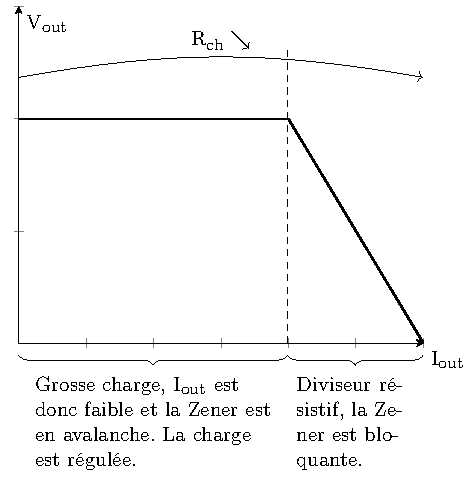
\includegraphics[]{zener-vout-iout.pdf}
%\end{center}
%
%Déterminons l'équation de la droite décroissante~: $V_{out} = V_2 \cdot \frac{R_{ch}}{R + R_{ch}}$ et $V_{out} = R_{ch} \cdot I_{out}$. Ainsi, $R_{ch} = \frac{V_{out}}{I_{out}}$, et donc $V_{out} = V_2 \cdot \frac{V_{out}/I_{out}}{R+ V_{out}/I_{out}} = V_2 \cdot \frac{V_{out}}{R\cdot I_{out} + V_{out}} \Leftrightarrow V_2 = R\cdot I_{out} + V_{out} \Leftrightarrow V_{out} = V_2 - R\cdot I_{out}$.
%
%}%R
	%\label{Q:24}
%
%
%\Question
%{
	%Établissez l'expression du rendement du montage en fonction de $I_{out}$.
	%%
	%Discutez le résultat obtenu.
%}
%{
%$\eta = \frac{P_{out}}{P_{in}} = \frac{P_{ch}}{P_{V2}} = \frac{R_{ch} \cdot I_{out}^2}{V_2 \cdot I} = \frac{R_{ch} \cdot I_{out}^2}{V_2 \cdot \frac{V_2 - V_z}{R}}
%$
%}%R
	%\label{Q:25}
%
%\vspace{-0.5cm}
%
%\subsection{Manipulation}
%\Question
%{
	%Ajoutez le régulateur de tension à la sortie de votre montage.
%}
%{}%R
	%\label{Q:26}
%
%\Question
%{
	%Tracez la caractéristique de sortie du circuit $I_{out} = f(V
	%_{out})$ en relevant les points de fonctionnement pour différentes valeurs de résistance de charge.
%
%
	%Déterminez ensuite l'expression générale de la droite du charge du montage complet $I_z = f(V_z, R, R_{ch}, V_2)$.
%
	%\textit{Aide~:} Posez clairement les équations de maille, nœud et constitutives du montage, puis exprimez $I_z$ en fonction des autres grandeurs.
%
	%% Tracez enfin différentes droites de charge sur la caractéristique $I_z = f(V_z)$ donnée ci-dessous.
	%% \begin{center}
	%% 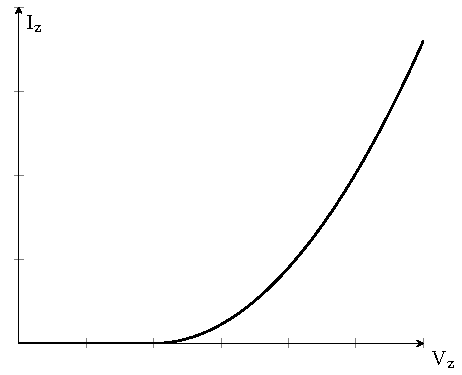
\includegraphics[]{zener-carac-seule.pdf}
	%% \end{center}
%}
%{
%\begin{center}
%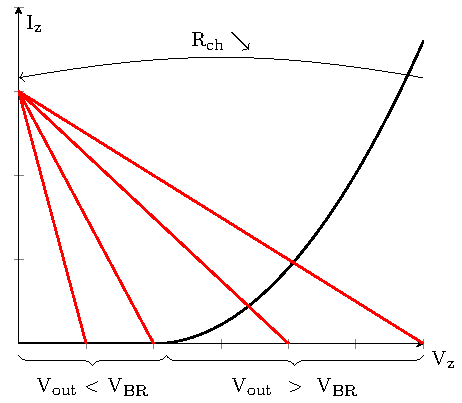
\includegraphics[]{zener-carac-charge.pdf}
%\end{center}
%
%Déterminons l'équation des différentes droites de charge tracées en rouge ci-dessus.
%
%\[	\begin{cases}
	%V_2 - V_R - V_z = 0 \Leftrightarrow V_R = V_2 - V_z\\
	%V_z = V_{out} \\
	%V_R = i \cdot R \Leftrightarrow i = \frac{V_R}{R}\\
	%V_{out} = i_{out} \cdot R_{ch} \Leftrightarrow i_{out} = \frac{V_{out}}{R_{ch}}\\
	%i = i_z + i_{out} \Leftrightarrow i_z = i - i{out} = \frac{V_2 - V_z}{R} - \frac{V_z}{R_{ch}}\\
	%\end{cases}
%\]
%
%En mettant $V_z$ en évidence dans cette dernière relation, on retrouve bien l'équation d'une droite de pente négative avec une ordonnée à l'origine positive.
%
%\[I_z = - \frac{R + R_{ch}}{R \cdot R_{ch}} \cdot V_z + \frac{V_2}{R}\]
%
%On peut à nouveau constater que lorsque la charge $R_{ch}$ diminue, le point de fonctionnement se trouve dans la zone bloquante de la diode zener.
%Elle n'assure dès lors plus son rôle de régulation, aucun courant $I_z$ ne la traverse et le montage se réduit à un simple diviseur résistif.
%
%
%
%}%R
	%\label{Q:27}

\end{document}
